\section{Architecture of CAIS}\label{sec:cais_architecture}

In this section, we provide an overview of the general architecture that a
CAIS should follow for its implementation. From our experience, we believe
that the ideal architecture is one that is principally event-driven and
modular. By modular, we mean that each component of the system
should be implemented as a separate piece, following the UNIX philosophy for composable programs of 
``doing one thing and doing it well''~\cite{mcilroy_unix_1978}. The advantage of
this approach is that it allows one to easily substitute out pieces that with
something else, or not include them at all where it makes sense.
Figure~\ref{fig:cais_high_level} shows this concept for the input and output
layers of the CAIS. As shown, we show each piece of input hardware flowing
into its own worker module. The worker module is then tasked with turning the
raw input into something meaningful before it is passed along to be fused
with the other input mechanisms. In this way, the CAIS is responsible for
dealing with the fusion of sensors and that it is flexible in that not
all paths may be utilized.

\begin{figure}
    \centering
    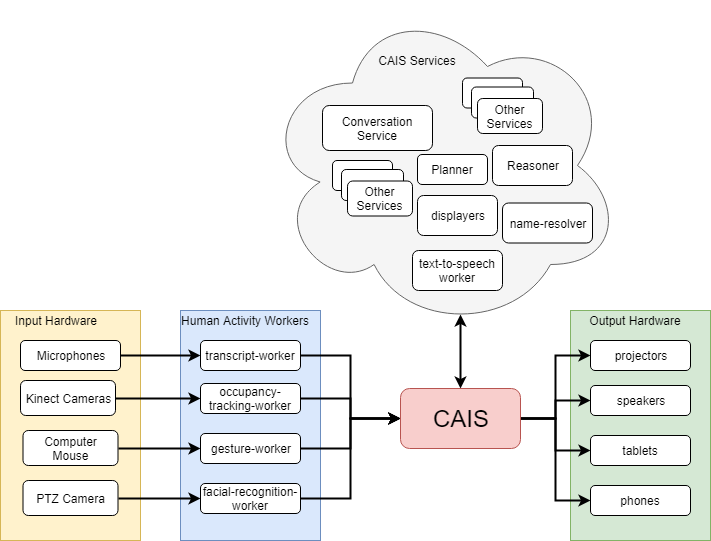
\includegraphics[width=0.5\columnwidth]{chapters/02_technology/figures/cais_high_level.png}
    \caption{High level diagram of CAIS architecture.}
    \label{fig:cais_high_level}
\end{figure}

As stated above, the architecture here is event-driven, such that workers can
be activated at any time, and then feeds through the CAIS, triggering further
modules as the event is fed forward. For example, the transcript-worker is
activated with the event of someone talking into the system. Important to
this model is the communication methods which we utilize within our system.
Principally, we utilize a distributed message queue wherein modules can
register as producers and consumers, allowing messages to be passed, which
act as the events of the system. One of the requirements here is that we
expect that multiple modules may consume from the same producer, allowing
a singular event to trigger multiple pieces downstream. Generally, each
``core'' module of the CAIS acts as both a producer and consumer, with
the exception of the edge modules, such that input modules (e.g. 
transcript-worker) are producers and the output modules (e.g. speaker-worker)
are consumers. For our purposes here, we utilize 
RabbitMQ~\cite{pivotal_software_rabbitmq_2020}, a commercially available
message broker that fits our needs. To accomplish the above message queue
requirement With RabbitMQ, we utilize a broadcast model where modules
subscribe to event topics, where each topic is made up of a number of pieces. 
Each topic is
unique to a given event, and that the topic pieces are specified in a manner of
least specific (e.g. the module name) to most specific (e.g. the event action).
Any number of consumers can subscribe to a given topic, each receiving the same
event. For example, the transcript-worker produces output on the topic
``transcript.result.interim'' (for in-progress speech transcription) and
``transcript.result.final'' (for finished speech transcription). Any number of
consumers could then listen to either of those channels, and be activated by
a transcription event. In rare cases, certain modules utilize RPC communication,
principally for modules that are hooked to a specific hardware device (e.g.
speaker-worker which is connected to a system's speakers). However, it's
expected that while communication to the module itself is done via a single RPC
queue, the module then broadcasts out events relating to what it is doing. For
the speaker-worker, this means that it will receive a sentence to output
via the speakers, and it will issue an event ``speaker.speak.begin'' before
it starts playing the sound, and ``speaker.speak.end'' when it finishes, which
any module can subscribe to.

Finally, for services that are not necessarily core to the CAIS itself, but
rather contain information or outside capabilities, we largely rely upon
utilizing standard TCP calls to these services. These services are, but not
limited to, things like databases, prover, external APIs.

A limitation of this approach is that each new link between modules introduces
additional latency to the system. However, within everything running on a high
speed connection, the added latency is roughly ~8ms per link. This throughout
is not largely felt by the user over the bottleneck of slower operations
involved with calling some of the external services and complex operations
of the CAIS, such as transcription service for parsing microphone input.

We are confident in our approach, and are in good company with  prior work that
followed a similar approach, such as the work done by
Brooks~\cite{brooks_intelligent_1997}. However, unlike this prior work, through
the use of RabbitMQ, the links between modules are that of topics, and not
necessarily hard coded agent links.
